\documentclass[12pt,english,dvipsnames,aspectratio=169,handout]{beamer}\usepackage[]{graphicx}\usepackage[]{xcolor}
% maxwidth is the original width if it is less than linewidth
% otherwise use linewidth (to make sure the graphics do not exceed the margin)
\makeatletter
\def\maxwidth{ %
  \ifdim\Gin@nat@width>\linewidth
    \linewidth
  \else
    \Gin@nat@width
  \fi
}
\makeatother

\definecolor{fgcolor}{rgb}{0.345, 0.345, 0.345}
\newcommand{\hlnum}[1]{\textcolor[rgb]{0.686,0.059,0.569}{#1}}%
\newcommand{\hlstr}[1]{\textcolor[rgb]{0.192,0.494,0.8}{#1}}%
\newcommand{\hlcom}[1]{\textcolor[rgb]{0.678,0.584,0.686}{\textit{#1}}}%
\newcommand{\hlopt}[1]{\textcolor[rgb]{0,0,0}{#1}}%
\newcommand{\hlstd}[1]{\textcolor[rgb]{0.345,0.345,0.345}{#1}}%
\newcommand{\hlkwa}[1]{\textcolor[rgb]{0.161,0.373,0.58}{\textbf{#1}}}%
\newcommand{\hlkwb}[1]{\textcolor[rgb]{0.69,0.353,0.396}{#1}}%
\newcommand{\hlkwc}[1]{\textcolor[rgb]{0.333,0.667,0.333}{#1}}%
\newcommand{\hlkwd}[1]{\textcolor[rgb]{0.737,0.353,0.396}{\textbf{#1}}}%
\let\hlipl\hlkwb

\usepackage{framed}
\makeatletter
\newenvironment{kframe}{%
 \def\at@end@of@kframe{}%
 \ifinner\ifhmode%
  \def\at@end@of@kframe{\end{minipage}}%
  \begin{minipage}{\columnwidth}%
 \fi\fi%
 \def\FrameCommand##1{\hskip\@totalleftmargin \hskip-\fboxsep
 \colorbox{shadecolor}{##1}\hskip-\fboxsep
     % There is no \\@totalrightmargin, so:
     \hskip-\linewidth \hskip-\@totalleftmargin \hskip\columnwidth}%
 \MakeFramed {\advance\hsize-\width
   \@totalleftmargin\z@ \linewidth\hsize
   \@setminipage}}%
 {\par\unskip\endMakeFramed%
 \at@end@of@kframe}
\makeatother

\definecolor{shadecolor}{rgb}{.97, .97, .97}
\definecolor{messagecolor}{rgb}{0, 0, 0}
\definecolor{warningcolor}{rgb}{1, 0, 1}
\definecolor{errorcolor}{rgb}{1, 0, 0}
\newenvironment{knitrout}{}{} % an empty environment to be redefined in TeX

\usepackage{alltt}
\usepackage{fontspec}
\setsansfont[Mapping=tex-text]{Fira Sans}
\setcounter{secnumdepth}{4}
\setcounter{tocdepth}{4}
\usepackage[normalem]{ulem}
\usepackage[T1]{fontenc}
\usepackage{dcolumn}
\usepackage{booktabs}
\usepackage{bm}
\usepackage{setspace}
\makeatletter
\usetheme{metropolis}
\setbeamertemplate{frame footer}{Bosancianu | Schaub | Hertie School}
\setbeamerfont{page number in head/foot}{size=\tiny}
\setbeamercolor{footline}{fg=gray}
\usepackage{xcolor}
\usepackage{tikz}
\usetikzlibrary{arrows, positioning}
\usepackage[labelformat=empty]{caption}
% For table captions in Beamer
\usepackage[sectionbib]{apacite}
\renewcommand{\bibliographytypesize}{\footnotesize}
\makeatletter
\let\st@rtbibsection\@bibnewpage
\let\st@rtbibchapter\@bibnewpage
\makeatother
\usepackage{amsmath, mathtools}
\usepackage{xunicode}
\usepackage{hyperref}
\graphicspath{{./figures/}} 
% Defines a checkmark
\def\checkmark{\tikz\fill[scale=0.4,color=orange](0,.35) -- (.25,0) -- (1,.7) -- (.25,.15) -- cycle;}
% wide itemize and enumerate
\newenvironment{wideitemize}{\itemize\addtolength{\itemsep}{.3em}}{\enditemize}
\newenvironment{wideenumerate}{\enumerate\addtolength{\itemsep}{.3em}}{\endenumerate}
% boxes
\def\boxitorange#1{%
  \smash{\color{orange}\fboxrule=1pt\relax\fboxsep=2pt\relax%
  \llap{\rlap{\fbox{\vphantom{0}\makebox[#1]{}}}~}}\ignorespaces
}
\def\boxitblue#1{%
  \smash{\color{blue}\fboxrule=1pt\relax\fboxsep=2pt\relax%
  \llap{\rlap{\fbox{\vphantom{0}\makebox[#1]{}}}~}}\ignorespaces
}
\newcommand{\indep}{\perp \!\!\!\! \perp}
\setbeamertemplate{itemize items}{\checkmark}
\usepackage{multirow}
\hypersetup{pdfauthor={Bosancianu and Schaub},
	pdftitle={Statistical Modeling and Causal Inference with R},
	pdfsubject={Week 3: Revisiting regression estimators of causal effects},
	pdfkeywords={Berlin, Hertie, 2020, week 3}}
\title{\textsc{Statistical Modeling and Causal Inference with R}}
\subtitle{Week 3: Revisiting regression estimators of causal effects}
\date{September 21, 2020}
\author{Manuel Bosancianu \hfill Max Schaub}
\institute{Hertie School of Governance}
\IfFileExists{upquote.sty}{\usepackage{upquote}}{}
\begin{document}
\maketitle


\begin{frame}
	\frametitle{Today's focus}
	
	\begin{itemize}
		\item Recap: Motivation for causal inference (CI)
		\item Ordinary Least Square Regression (OLS)
		\item Regression and the potential outcomes framework (POF)
		\item Regression as a tool to reduce omitted variable bias (OVB)
	\end{itemize}
	
\end{frame}

\section{Recap: Motivation for causal inference (CI)}


\begin{frame}
	\frametitle{Motivation for CI}
	
	\begin{itemize}
		\setlength\itemsep{1.5em}
		\item How to ``get from raw numbers to reliable causal knowledge''? \cite[xiii]{angrist_mastering_2015}
		\item How to get to \emph{ceteris paribus} / all other things equal condition?
	\end{itemize}
	
\end{frame}


\begin{frame}
	\frametitle{Motivation for CI}
	
	\begin{itemize}
		\item More formally, we are after estimating the difference between a control and a treatment group
		\item Due to the `fundamental problem of causal inference' \cite{holland_statistics_1986}, we only ever observe individuals either in their treated $Y_{1i}|D_i=1$ or their untreated $Y_{0i}|D_i=0$ state
		\item We do not observe the counterfactuals $Y_{1i}|D_i=0$ (the potential outcome of the treated had they not received the treatment) and $Y_{0i}|D_i=1$, the outcome of the non-treated had they been treated
	\end{itemize}
	
\end{frame}


\begin{frame}
	\frametitle{Motivation for CI}
	
	\begin{itemize}
		\item The naive comparison (the NATE) in non-experimental settings is therefore very likely biased
    \item Using the constant-effect assumption $Y_{1i}= Y_{0i} + \kappa$ (i.e. assuming no heterogeneous treatment effect (HTE) bias) we can identify the selection bias as follows:
	\end{itemize}
	\begin{equation}
  \begin{split}
  NATE 	& = E[Y_{1i}|D_i=1] - E[Y_{0i}|D_i=0]\\
		& = E[Y_{0i} + \kappa |D_i=1] - E[Y_{0i}|D_i=0]\\
		& = \kappa + \textcolor{orange}{{E[Y_{0i}|D_i=1] - E[Y_{0i}|D_i=0]}}\\
  \end{split}
\end{equation}

\end{frame}


\begin{frame}
	\frametitle{Motivation for CI}
	
	\begin{itemize}
		\setlength\itemsep{1.5em}
		\item The term $E[Y_{0i}|D_i=1] - E[Y_{0i}|D_i=0]$ is the selection bias: \emph{everything} that distinguishes the treatment group from the control group in their non-treated states
		\item \textcolor{orange}{The principal goal of CI methods is the elimination of the selection bias}
	\end{itemize}
	
\end{frame}




\section{Ordinary Least Square Regression (OLS)}

\begin{frame}
  \frametitle{Ordinary Least Square Regression \emph{aka} Regression}
	\begin{itemize}
		\item What does regression do?  
		\item Simple regression: look for the best linear approximation of the relationship between two variables ($\rightarrow$ \href{https://students.brown.edu/seeing-theory/regression-analysis/index.html}{link to interactive visualization})
	\end {itemize}
	 \begin{figure} 
    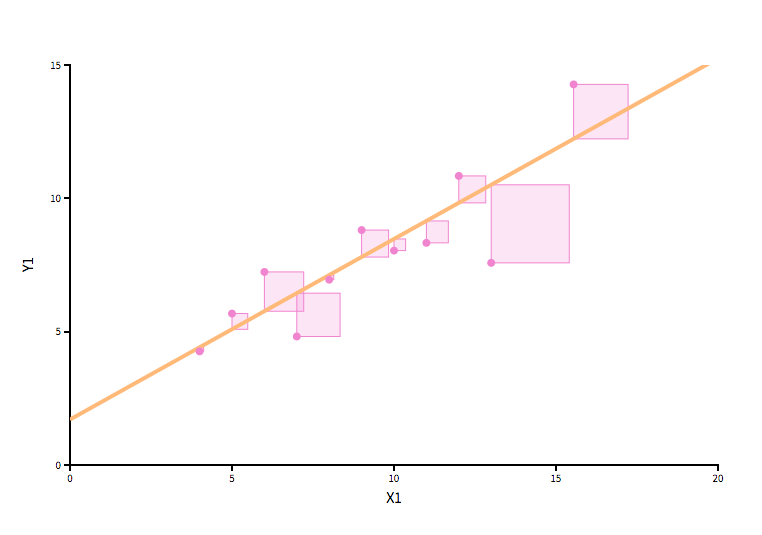
\includegraphics[height=.5\textheight]{../04-figures/03/01-simple_ols}
    \end{figure}
    
\end{frame}


\begin{frame}
\frametitle{Ordinary Least Square Regression \emph{aka} Regression}

\begin{itemize}
	\item Best fitting line is found by minimizing the sum of the squared deviations from a line 
  \item OLS regression is a solution to an optimization problem:
	\end {itemize}
  \begin{center}
  $Y_{i} = \beta_{0} + \beta_{1}X + r_{i}$ \\
  $\sum_{i=1}r_{i}^{2} = \text{min}$
  \end{center}
  \pause
\begin{itemize}
		\item \textcolor{orange}{How does this relate to causal inference?}
	\end {itemize}
	
\end{frame}


\begin{frame}
\frametitle{Regression as a descriptive tool}

\begin{itemize}
    \item Regression may be justified without any reference to causality: as a method for obtaining a best-fitting linear descriptive model of $Y$ given $X$ -- the conditional expectation function (CEF)  $E(Y|X)$
    \item The focus here is on \textcolor{orange}{predicting} Y given specific realizations of $X$
    \item Under this use of regression, the outcome $Y$ is not generally thought to be a function of potential outcomes associated with causal states
    \item \textcolor{orange}{No close link between this use of regression and CI; inappropriate to give a causal interpretation to any of the estimated regression coefficients} 
  \end{itemize}
  
\end{frame}


\begin{frame}
\frametitle{Regression as a tool for causal inference}

\begin{itemize}
  \item But often, regression models \textcolor{orange}{are} used to do causal inference! When is this justified?
  \item Regression can be used to estimate quantities you know from the potential outcomes framework (POF)
  \item Notably, 
    \begin{enumerate}
      \item The individual treatment effect $ITE = Y_{1i} - Y_{0i}$ can be expressed as a regression equation
      \item The selection bias is intimately linked with the error term (often written as $u_i$ or $e_i$)
      \item Controlling for potential confounders is a way to reduce selection bias
    \end{enumerate}
\end{itemize}

\end{frame}




\section{Regression and the potential outcomes framework (POF)}


\begin{frame}
\frametitle{Regression and the POF}

1. The individual treatment effect (ITE) and the regression equation:

\small
  \begin{align*}
Y_i &= D_i Y_{1i} + (1-D_i) Y_{0i} & \text{\scriptsize switching equation} \\
		% says that outcome is either observed in its treated or it's untreated state
		&=D_i Y_{1i} + Y_{0i} - D_i Y_{0i} & \text{\scriptsize rearrange} \\
		&= Y_{0i} + D_i(Y_{1i} - Y_{0i}) & \text{\scriptsize add $E[Y_{0i}] - E[Y_{0i}]$, rearrange} \\
		&= Y_{0i} + D_i(Y_{1i} - Y_{0i}) + E[Y_{0i}] - E[Y_{0i}] &  	\text{\scriptsize use $Y_{1i}= Y_{0i} + \kappa$, rearrange}	\\
		&= E[Y_{0i}] + \kappa D_i + Y_{0i} - E[Y_{0i}] & \text{\scriptsize simplify terms} \\
Y_i	&=\underbrace{\alpha}_{\textrm{$E[Y_{0i}]$}} + \underbrace{\kappa}_{\textrm{$Y_{1i} - Y_{0i}$}}D_i + \underbrace{u_i}_{\textrm{$Y_{0i} - E[Y_{0i}]$}} & \text{\scriptsize the classic regression equation!}
  \end{align*}

\end{frame}


\begin{frame}

\frametitle{Regression and the POF}

2. The error term and selection bias:

Evaluating the conditional expectation of this equation with treatment switched off and on allows us to see the connection between the error term of the regression and selection bias:

  \begin{align*}
    E[Y_{1i}|D = 1] &= \alpha + \kappa +  E[u_i|D = 1]\\
    E[Y_{0i}|D = 0] &= \alpha + E[u_i|D = 0]\\
  \shortintertext{ after deducting the above from each other, we get:}
\underbrace{E[Y_{1i}|D = 1] - E[Y_{0i}|D = 0]}_{\textrm{NATE}} &=\underbrace{\kappa}_{\textrm{ATE}} + E[u_i|D = 1] - E[u_i|D = 0]\\
\end{align*}

\end{frame}



\begin{frame}
\frametitle{Regression and the POF}

\begin{flushleft}
2. The error term and selection bias:
\end{flushleft}

Since $u_i = Y_{0i} - E[Y_{0i}]$, we can rewrite the last term:

{\centering
  $ \displaystyle
    \begin{aligned} 
    E[u_i|D = 1] - E[u_i|D = 0] &= E[Y_{i0}|D = 1] - E[Y_{i0}|D = 0] \\
    \end{aligned}
  $ 
\par}  

\begin{flushleft}
which gives us:
\end{flushleft}

{\centering
  $ \displaystyle
    \begin{aligned} 
\small \underbrace{E[Y_{1i}|D = 1] - E[Y_{0i}|D = 0]}_{\textrm{NATE}} &= \small\underbrace{\kappa}_{\textrm{ATE}} + \underbrace{E[Y_{i0}|D = 1] - E[Y_{i0}|D = 0]}_{\textrm{Selection bias}}\\
    \end{aligned}
  $ 
\par}
\vspace{3mm}
This means the regression equation recovers the ATE if it's not affected by selection bias.

\end{frame}


\begin{frame}
\frametitle{Regression and the POF}

2. The error term and selection bias:

Going back to the regression equation notation of the causal outcomes, i.e.\  $Y_i = \alpha + \kappa D_i + u_i$, the unbiasedness requirement can also be expressed as the the conditional mean zero
  requirement for the error term: \textcolor{orange}{$E[u_i|D_i] = 0$}. 
  
  This means that for $\kappa$ to capture the causal effect of the treatment $D_i$, the error has to be independent from the treatment, or, in other words, treatment assignment has to be unaffected by selection bias.

\end{frame}



\begin{frame}
\frametitle{Regression and the POF}

3. Controlling for confounders as a way to reduce selection bias

\begin{itemize}
  \item Why bother using the regression framework for causal inference, if the problem of the regression estimator is the same as with the naive estimator?
  \item Multiple regression allows to control for other variables: this can help to reduce (or even remove) selection bias
  \item The multiple regression function can be written as
  \begin{align*}
  Y_i &= \beta_0 + \beta_1 X_i + \beta_2 W_i + \ldots + \beta_n Z_i + u_i \\
  \shortintertext{or sticking with our notation as:}
  Y_i &= \alpha + \kappa D_i + \beta W_i + u_i
  \end{align*}
\end{itemize}

\end{frame}




\begin{frame}
\frametitle{Regression and the POF}

3. Controlling for confounders as a way to reduce selection bias

\small
Think of $W_i$ as an additional factor that we know or assume to influence the relationship between the treatment and the outcome. 

Example 1: In an experimental setting, we might know that one group had a higher chance of receiving a treatment. E.g.\ an experiment that involved randomly distributing loans where the implementing micro-finance company insisted that 70\% of participants had to be female. 

\end{frame}




\begin{frame}
\frametitle{Regression and the POF}

3. Controlling for confounders as a way to reduce selection bias

\small
Example 2: In an observational study, where we are interested in the effect of contact on prejudice, $W_i$ could stand for education, as it is plausible that the educated are both more likely to seek out contact and to hold lower prejudice.

Using the benchmark of the ideal experiment, we can think of these factors as devitations from random assignment: women/the educated are more likely to receive the treatment.

If we don't take into account this deviation, this would mean that treatment assignment is no longer independent of the error term $E[u_i|D_i] \neq 0$ -- our estimate for the causal effect is biased.

\end{frame}



\begin{frame}
\frametitle{Regression and the POF}

3. Controlling for confounders as a way to reduce selection bias

How does controlling for $W_i$ affect our estimates?

Conditional on $W_i$, the treatment assignment becomes independent of the error term again:

$E[u_i|D_i,W_i] = E[u_i|W_i]$

\small (but note that the same is not true for the confounder $W_i$, i.e.\ $E[u_i|W_i] \neq 0$ -- this is one reason why you should only ever focus strictly on one variable during a given analysis).

\end{frame}



\begin{frame}
\frametitle{Regression and the POF}

3. Controlling for confounders as a way to reduce selection bias

We can see this by evaluating the conditional expectation of the multiple regression equation:
  \begin{align*}
  \scriptstyle Y_i                     &= \scriptstyle \alpha + \kappa D_i + \beta W_i + u_i \\
  \scriptstyle E[Y_i|D=1]              &= \scriptstyle \alpha + \kappa + \beta W_i + E[u_i|D_i=1, W_i] \\
  \scriptstyle E[Y_i|D=0]              &= \scriptstyle \alpha + \beta W_i + E[u_i|D_i=0, W_i] \\
  \shortintertext{\footnotesize deduct from each other and resolve:}
  \scriptstyle E[Y_i|D=1] - E[Y_i|D=0] &= \scriptstyle \kappa + E[u_i|D_i=1, W_i] -  E[u_i|D_i=0, W_i] \\
  \scriptstyle E[Y_i|D=1] - E[Y_i|D=0] &= \scriptstyle \kappa + E[u_i| W_i] -  E[u_i| W_i] \\
  \scriptstyle E[Y_i|D=1] - E[Y_i|D=0] &= \scriptstyle \kappa 
  \end{align*}

\end{frame}



\section{Regression as a tool to reduce omitted variable bias (OVB)}


\begin{frame}
\frametitle{Regression as a tool to reduce OVB}

Under a causal inference perpective, the use of regression is to \textcolor{orange}{minimize the influence of confounders} that can cause selection bias in our estimate of the causal effect.

In other words, we aim to make our treatment variable \textcolor{orange}{condionally independent} of the error term.

In yet other words, we aim to make our treatment \textcolor{orange}{ignorable}.

And in yet other words, in CI we use regression to \textcolor{orange}{minimize omitted variable bias (OVB)}.

\end{frame}


\begin{frame}
\frametitle{Regression as a tool to reduce OVB: Example}

Your starting points for a causally minded regression analysis are: 
\begin{itemize}
  \item A clear \textcolor{orange}{hypothesis} that formulates an outcome and a treatment
  \item \textcolor{orange}{Data} including measures for treatment, outcome and potential confounders
  \item A \textcolor{orange}{causal model} detailing how all factors interact, e.g.\ in the form of a directed acyclic graph (DAG) -- much more on this in the next session
  \item A \textcolor{orange}{statistical model} / regression equation
\end{itemize}

\end{frame}

\begin{frame}
\frametitle{Regression as a tool to reduce OVB: Example}

Here: 
\begin{itemize}
  \item Hypothesis: Church attendance reduces belief in anthropogenic global warming
    \begin{itemize} \footnotesize
      \item Doubtful of humans as cause of global developments
      \item Influence of preachers critical of global warming
      \item \ldots
    \end{itemize} \normalsize
  \item Data from Egan and Mullin \citeyear{egan_turning_2012}
  \item Causal model:
    \begin{figure}
    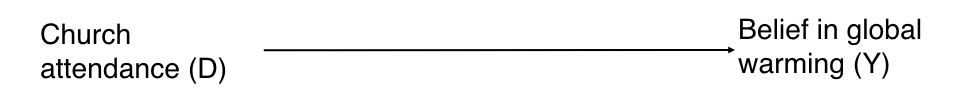
\includegraphics[width=0.75\textwidth]{../04-figures/03/02-w3_dag1}
    \end{figure}
  \item Statistical model: $Y_i = \alpha + \kappa D_i + u_i$
\end{itemize}

\end{frame}


\begin{frame}
\frametitle{Regression as a tool to reduce OVB: Example}

Note a few things:

\begin{itemize}
  \item The setting does not approximate an experiment in any way 
      \begin{itemize} \footnotesize
      \item no random assignment, but individual choice
      \item hard to know who goes to church and why
      \item a lot of potential confounders 
      \end{itemize} \normalsize
  \item This should make you extra cautious and pay careful attention to the explanation as to how the causal effect is to be recovered
  \item Similarly difficult-to-test hypotheses are tested all the time in published research -- some of them with good identification strategies, some (many) with bad ones
\end{itemize}

\end{frame}


\begin{frame}
\frametitle{Regression as a tool to reduce OVB: Example}

Let's first look at the data: 

\scriptsize
\begin{table}[htbp]\centering
\begin{tabular}{l*{1}{lccc}}
\toprule
                                             &\multicolumn{4}{c}{}                   \\
                                             &     mean&       sd&      min&      max\\
\midrule
Earth getting warmer?                        &     0.79&     0.40&        0&        1\\
Attends church                               &     0.89&     0.32&        0&        1\\
Sex: Male                                    &     0.48&     0.50&        0&        1\\
Party ID: Republican                         &     0.30&     0.46&        0&        1\\
Departure from normal local temperature      &         &         &        &          \\
(in 10 \textdegree F) in week prior to survey           &     0.38&     0.59&       -2&    4\\
\bottomrule
\end{tabular}
\caption{\scriptsize Summary statistics for selected variables from Egan and Mullin \citeyear{egan_turning_2012}}
\end{table}

\end{frame}



\begin{frame}
\frametitle{Regression as a tool to reduce OVB: Example}

Regression results estimating  $Y_i = \alpha + \kappa D_i + u_i$: 

\scriptsize
\begin{table}
\begin{center}
\begin{tabular}{l D{.}{.}{4.6}}
\toprule
 & \multicolumn{1}{c}{Naive Model} \\
\midrule
(Intercept) & 0.950^{***}  \\
            & (0.030)      \\
Attends church  & -0.082^{***} \\
            & (0.016)      \\
\midrule
R$^2$       & 0.004        \\
Num. obs.   & 6219         \\
\bottomrule
\multicolumn{2}{l}{\tiny{$^{***}p<0.001$; $^{**}p<0.01$; $^{*}p<0.05$}}
\end{tabular}
\caption{\scriptsize Effect of church attendance on belief in anthropogenic climate change}
\label{table:coefficients}
\end{center}
\end{table}

\end{frame}

\begin{frame}
\frametitle{Regression as a tool to reduce OVB: Example}

How credible is this result? Is 8.2\% a good estimate for the causal effect? Is the estimate free from confounding? That is, is `treatment assignment' uncorrelated with the error term, i.e.\ $E[u_i|D_i] = 0$?
\pause
Many possible confounders, e.g.\ ideology:

    \begin{figure}
    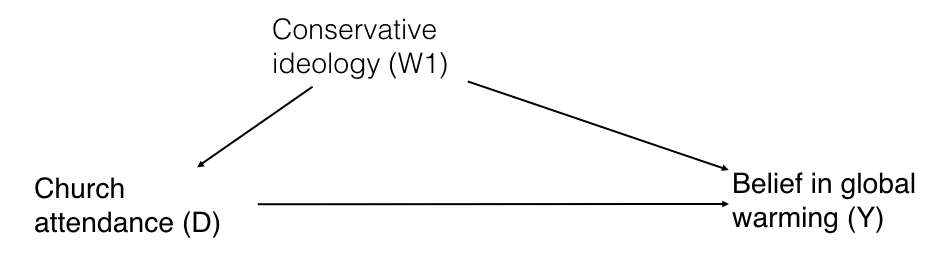
\includegraphics[width=0.75\textwidth]{../04-figures/03/03-w3_dag2a}
    \end{figure}
    
How does the failure to control for ideology bias our results?

\end{frame}


\begin{frame}
\frametitle{Regression as a tool to reduce OVB}

\footnotesize
To find out, we analyze omitted variable bias -- the difference in the causal effect when controlling for the confounder (the `long regression') as compared to when not controlling for it (the `short regression'), which is captured by the following formula \cite{angrist_mastering_2015}: 

\scriptsize
OVB = \{Relationship between potential confounder and proposed treatment variable\} $\times$ \{Effect of potential confounder in long regression\} 

\footnotesize
Given the three regressions
\vspace{-2mm}
\begin{align*}
    Y_i &= \alpha^s + \kappa^s D_i + u_i^s\;\text{\footnotesize  (short)} \\
    Y_i &= \alpha^l + \kappa^l D_i + \beta W_i + u_i^l\;\text{\footnotesize  (long)} \\
    W_i &= \theta + \gamma D_i + e_i\;\text{\footnotesize (relationship confounder and treatment)}
    \shortintertext{the OVB is calculated as:}
OVB &= \kappa^s - \kappa^l  = \gamma \times \beta \nonumber
\end{align*}

\end{frame}


\begin{frame}
\frametitle{Regression as a tool to reduce OVB}

The OVB formula is a heuristic tool for gauging the presence and direction of the selection bias. 

It's most useful when you cannot actually observe a confounder but want to determine its likely effect.

\footnotesize
\vspace{5mm}
\textcolor{orange}{When does OVB become zero}? I.e.\ $\kappa^s - \kappa^l  = \gamma \times \beta = 0$?

\begin{enumerate}
  \item $\beta=0$ (\footnotesize no effect of confounder on outcome \normalsize)
  \item $cov(D_i, W_i)=0$ (\footnotesize treatment and confounder actually independent\normalsize)
\end{enumerate}

\end{frame}


\begin{frame}
\frametitle{Regression as a tool to reduce OVB}

\footnotesize
\textcolor{orange}{When is OVB negative}? I.e.\ the estimate for the causal effect a) overestimates the true effect when the estimate for the causal effect is negative, b) underestimates the true effect when the estimate is positive: $\kappa^s - \kappa^l  = \gamma \times \beta < 0$? 

\begin{enumerate}
  \item $\gamma$ and $\beta$ take different signs 
\end{enumerate}

\textcolor{orange}{When is OVB positive}? I.e.\ the estimate for the causal effect a) underestimates the true effect when the estimate for the causal effect is negative, b) overestimates the true effect when the estimate is positive: $\kappa^s - \kappa^l  = \gamma \times \beta > 0$?

\begin{enumerate}
  \item $\gamma$ and $\beta$ both positive  
  \item $\gamma$ and $\beta$ both negative 
\end{enumerate}

\end{frame}



\begin{frame}
\frametitle{Regression as a tool to reduce OVB: Example}

\footnotesize
In our example, is the effect of ideology on the outcome zero? Highly unlikely. And is the correlation between church attendance and ideology zero? Also highly unlikely. Estimates likely affected by OVB.

What is the likely direction of the bias?

What are the likely signs on the coefficients for $\beta$ and $\gamma$? (Hint: Use your DAG)
\vspace{-5mm}
\begin{align*} \footnotesize
    Y_i &= \alpha^l + \kappa^l D_i + \beta W_i + u_i^l\;\text{\footnotesize  (long)} \\
    W_i &= \theta + \gamma D_i + e_i\;\text{\footnotesize (relationship confounder and treatment)}
\end{align*}
 
\pause
    \begin{figure}
    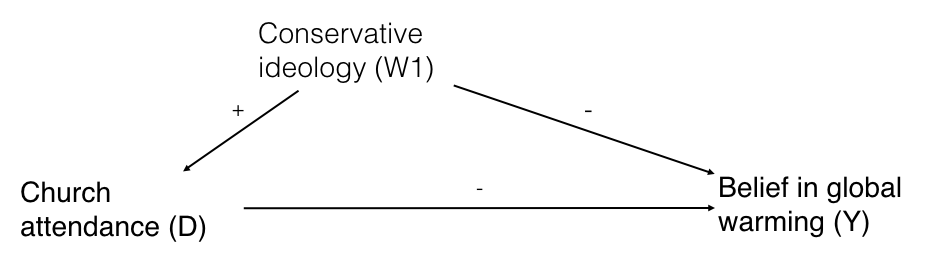
\includegraphics[width=0.6\textwidth]{../04-figures/03/04-w3_dag2b}
    \end{figure}

\end{frame}



\begin{frame}
\frametitle{Regression as a tool to reduce OVB: Example}

Our data provides a proxy for ideology, party ID, so we can actually check
\scriptsize

\begin{table}
\begin{center}
\begin{tabular}{l D{.}{.}{4.6} D{.}{.}{4.6} D{.}{.}{4.6}}
\toprule
 & \multicolumn{1}{c}{``Short'' Model} & \multicolumn{1}{c}{``Long'' Model} & \multicolumn{1}{c}{DV:RepID} \\
\midrule
(Intercept) & 0.950^{***}  & 0.955^{***}  & 0.029       \\
            & (0.030)      & (0.029)      & (0.033)     \\
Attends church  & -0.082^{***} & -0.050^{**}  & 0.141^{***} \\
            & (0.016)      & (0.016)      & (0.017)     \\
Party ID: Republican  &              & -0.228^{***} &             \\
            &              & (0.011)      &             \\
\midrule
R$^2$       & 0.004        & 0.069        & 0.010       \\
Num. obs.   & 6219         & 6219         & 6726        \\
\bottomrule
\multicolumn{4}{l}{\tiny{$^{***}p<0.001$; $^{**}p<0.01$; $^{*}p<0.05$}}
\end{tabular}
\caption{\scriptsize Effect of church attendance on belief in anthropogenic climate change}
\end{center}
\end{table}

\end{frame}


\begin{frame}
\frametitle{Regression as a tool to reduce OVB: Example}

\footnotesize
Estimate of OVB bias:
$\kappa^s - \kappa^l  = \gamma \times \beta = -0.082 - (-0.050) = −0.228 \times 0.141 = -0.032$

Estimate for $\kappa^s$ overestimates the effect of church attendance.

The strong change in coefficient is a clear warning sign: Ideology seems to be a highly important confounder, but is likely measured imperfectly with party ID.

This indicates that there are likely unobserved/unobservable variables influencing the estimate of $\kappa$. In other words, it remains doubtful that the `treatment' is independent from the error term, even when controlling for ideology, i.e.\ $E[u_i|D_i,W_i] \neq 0$ 

Unclear if this can be addressed with controls at all.

\end{frame}



\begin{frame}
\frametitle{Regression as a tool to reduce OVB: Example}

Further controls further reduce effect size

\tiny
\begin{table}
\begin{center}
\begin{tabular}{l D{.}{.}{4.6} D{.}{.}{4.6} D{.}{.}{4.6}}
\toprule
 & \multicolumn{1}{c}{``Short'' Model} & \multicolumn{1}{c}{``Long'' Model} & \multicolumn{1}{c}{``Controlled'' Model} \\
\midrule
(Intercept)        & 0.950^{***}  & 0.955^{***}  & 0.963^{***}  \\
                   & (0.030)      & (0.029)      & (0.030)      \\
Attends church         & -0.082^{***} & -0.050^{**}  & -0.036^{*}   \\
                   & (0.016)      & (0.016)      & (0.015)      \\
Party ID: Republican         &              & -0.228^{***} & -0.202^{***} \\
                   &              & (0.011)      & (0.012)      \\
Party ID: leans Republican     &              &              & -0.130^{***} \\
                   &              &              & (0.016)      \\
Self-rating: very conservative       &              &              & -0.166^{***} \\
                   &              &              & (0.021)      \\
Self-rating: conservative &              &              & -0.074^{***} \\
                   &              &              & (0.012)      \\
Self-rating: liberal      &              &              & 0.040^{**}   \\
                   &              &              & (0.015)      \\
\midrule
R$^2$              & 0.004        & 0.069        & 0.098        \\
Num. obs.          & 6219         & 6219         & 6219         \\
\bottomrule
\multicolumn{4}{l}{\tiny{$^{***}p<0.001$; $^{**}p<0.01$; $^{*}p<0.05$}}
\end{tabular}
\label{table:coefficients}
\end{center}
\end{table}

\end{frame}




\begin{frame}
\frametitle{Regression as a tool to reduce OVB}

Compare these results to the ones using the suggested treatment in Egan and Mullin \citeyear{egan_turning_2012} 

\tiny
\begin{table}
\begin{center}
\begin{tabular}{l D{.}{.}{4.6} D{.}{.}{4.6} D{.}{.}{4.6}}
\toprule
 & \multicolumn{1}{c}{``Short'' Model} & \multicolumn{1}{c}{``Long'' Model} & \multicolumn{1}{c}{``Controlled'' Model} \\
\midrule
(Intercept)        & 0.784^{***} & 0.853^{***}  & 0.888^{***}  \\
                   & (0.006)     & (0.007)      & (0.008)      \\
Departure from normal local temperature   &  & &  \\
(in 10 \textdegree F) in week prior to survey        & 0.028^{**}  & 0.021^{*}    & 0.022^{**}   \\
                   & (0.009)     & (0.008)      & (0.008)      \\
Party ID: Republican          &             & -0.230^{***} & -0.202^{***} \\
                   &             & (0.011)      & (0.012)      \\
Party ID: leans Republican     &             &              & -0.130^{***} \\
                   &             &              & (0.016)      \\
Self-rating: very conservative        &             &              & -0.168^{***} \\
                   &             &              & (0.021)      \\
Self-rating: conservative &             &              & -0.076^{***} \\
                   &             &              & (0.012)      \\
Self-rating: liberal       &             &              & 0.041^{**}   \\
                   &             &              & (0.015)      \\
\midrule
R$^2$              & 0.002       & 0.068        & 0.099        \\
Num. obs.          & 6219        & 6219         & 6219         \\
\multicolumn{4}{l}{\tiny{$^{***}p<0.001$; $^{**}p<0.01$; $^{*}p<0.05$}}
\end{tabular}
\end{center}
\end{table}

\end{frame}


\begin{frame}
\frametitle{Regression as a tool to reduce OVB: Final thoughts}

\footnotesize
Egan and Mullin \citeyear{egan_turning_2012} have a much better claim that their proposed treatment -- deviations from local temperatures -- may be quasi-randomly distributed, conditional on things like geographical regions.

Other studies study the effect of factors that are due to choices. In such studies, using controls to make the `treatment' independent of confounders  (a strategy dubbed `selection on observables') becomes much less credible (even though you should still read the study and judge for yourself).

The problem is that we are often interested in `treatments' that depend on individual choices (e.g.\ effect of education, vaccination, micro-finance,\ldots)!

\end{frame}


\begin{frame}
\frametitle{Regression as a tool to reduce OVB: Final thoughts}

\footnotesize
In such cases, very careful analyses are necessary, ideally involving causal graphs and detailed discussions of the direction of the biases that might be effecting the estimated effect.

Because `selection into treatment' will often depend on unobservable/unmeasurable confounders, it might not be possible to present a fully convincing argument based on `statistical control' alone.

In such cases, we will seek to/should use some of the design-based techniques such as instrumental variables or RDD. These techniques seek to isolate the more plausibly random part of the variation in our treatment, and use that part of the variation to predict the outcome. Many of these techniques build upon regression.

\end{frame}

% END
\begin{frame}
\begin{center}
    \LARGE Thank you for watching, and see you next Monday!
\end{center}
\end{frame}

% REFERENCES %

\begin{frame}
\frametitle{References}
\bibliographystyle{apacite}
\bibliography{../Bibliography}
\vspace{5cm}
\end{frame}

\end{document}
